\documentclass[11pt]{beamer}
\usetheme{Madrid}
\usepackage[utf8]{inputenc}

\usepackage{hyperref}
\usepackage{amsmath}
\usepackage{amsfonts}
\usepackage{amssymb}
\usepackage{graphicx}
\DeclareMathOperator {\argmin}{argmin}
\usepackage{algorithmic}
\usepackage{algorithm}
\usepackage{wrapfig}
\usepackage{subcaption}
\graphicspath{{.}}

\author[1]{Beck Amir, Marcc Teboulle}


\title{Fast Iterative Shrinkage-Thresholding Algorithm for Linear Inverse Problem}
% Informe o seu email de contato no comando a seguir
% Por exemplo, alcebiades.col@ufes.br
\newcommand{\email}{email}
\setbeamercovered{transparent}
\setbeamertemplate{navigation symbols}{}
%\logo{}
\institute[]{UBC Okanagan}
\date{\today}
\subject{MATH 590A}

% ---------------------------------------------------------
% Selecione um estilo de referência
\bibliographystyle{plain}

%\bibliographystyle{abbrv}
%\setbeamertemplate{bibliography item}{\insertbiblabel}
% ---------------------------------------------------------

% ---------------------------------------------------------
\newtheorem{remark}{Remark}
\newtheorem{assumption}{Assumption}

\begin{document}
    \begin{frame}
        \titlepage
    \end{frame}

    \begin{frame}{ToC}
        \tableofcontents
    \end{frame}

\section{Context and Introduction}
    \subsection{The Context}
        \begin{frame}{Sum of Two Functions}
            Consider a function $f$ that can be written into the sum of two functions. 
            \begin{align}
                \min_{x} g(x) + h(x)
            \end{align}  
            When $g(x)$ is Lipschitz smooth and $h(x)$, closed convex and proper, we can use Beck and Teboulle's FISTA algorithm. 
            \begin{itemize}
                \item [1.] The function $h$ can be nonsmooth. 
                \item [2.] Taking the proximal operator of $h$ has to be possible and easy to implement (More on that later).
                \item [3.] Under the right conditions, the FISTA algorithm converges with $\mathcal O(1/k^2)$. 
            \end{itemize}
        \end{frame}
        \begin{frame}{Contributions}
            \begin{itemize}
                \item [1.] In Beck's and Teboulle's paper\cite{paper:FISTA}, they popularized the use of Nesterov Momentum for nonsmooth functions. 
                \item [2.] Beck proved the convergence with the convexity assumption on $g, h$. 
                \item [3.] The FISTA algorithm is provably faster than the alternative algorithm: ISTA, TWIST. 
            \end{itemize}
        \end{frame}
        \begin{frame}{A Major Assumption}
            \begin{assumption}[Convex Smooth Nonsmooth with Bounded Minimizers]\label{assumption:1}
                We will assume that $g:\mathbb E\mapsto \mathbb R$ is \textbf{strongly smooth} with constant $L_g$ and $h:\mathbb E \mapsto \bar{\mathbb R}$ \textbf{is closed convex and proper}. We define $f := g + h$ to be the summed function and $\text{ri}\circ \text{dom}(g) \cap \text{ri}\circ \text{dom}(h) \neq \emptyset$. We also assume that a set of minimizers exists for the function $f$ and that the set is bounded. Denote the minimizer using $\bar x$. 
            \end{assumption}
            We refer to this as ``\textbf{Assumption A.1}''. 
        \end{frame}
        \begin{frame}{Lipschitz Smoothness}
            \begin{definition}[Strong Smoothness]\label{def:strong_smoothness}
                A differentiable function $g$ is called strongly smooth with a constant $\alpha$ then it satisfies: 
                \begin{align}
                    |g(y) - g(x) - 
                    \langle \nabla g(x), y - x
                    \rangle| \le \frac{\alpha}{2}\Vert x - y\Vert^2
                    \quad \forall x, y\in \mathbb E. 
                \end{align}    
            \end{definition}
            \begin{block}{Remark}
                When $g$ is convex, then the absolute value can be removed; the above condition is equivalent to: 
                \begin{align*}
                   \Vert \nabla g(x) - \nabla g(y)\Vert \le \alpha\Vert y - x \Vert\quad 
                   \forall x, y \in \mathbb E,
                \end{align*}
                we assume $\Vert \cdot\Vert$ is the euclidean norm for simplicity. It has been shown in Beck's book, theorem 5.8\cite{book:first_order_opt}. 
            \end{block}
        \end{frame}
    \subsection{The Proximal Operator}
        \begin{frame}{Proximal Operator Definition}
            \begin{definition}[The Proximal Operator]
                For a function $f$ with $\alpha \ge 0$, the proximal operator is defined as: 
                \begin{align*}
                    \text{prox}_{f, \alpha}(x) := 
                    \arg\min_{y}\left\lbrace
                        f(y) + \frac{1}{2\alpha} \Vert y - x\Vert^2
                    \right\rbrace. 
                \end{align*}
            \end{definition}  
            \begin{remark}
                The proximal operator is a singled-valued mapping when $f$ is convex, closed, and proper. 
            \end{remark}
        \end{frame}
        \begin{frame}{Proixmal Operator and Set Projections}
            Observe that when $f$ is an indicator function $\delta_Q$ defined as: 
            \begin{align*}
                \delta_Q(x) := 
                \begin{cases}
                    0 & x \in Q,
                    \\
                    \infty  & x \not \in Q, 
                \end{cases}
            \end{align*}
            the proximal operator of $\delta_Q$ is
            \begin{align*}
               \text{prox}_{\delta_Q, \alpha}(x)=\underset{y}{\text{argmin}}
               \left\lbrace
                    \delta_Q(y) + \frac{1}{\alpha}\Vert x - y\Vert^2
               \right\rbrace = \argmin_{y\in Q}\Vert x - y\Vert^2,
            \end{align*}
            it searches for the closest point to the set $Q$ for all $\alpha > 0$, and it is called a projection. When $Q\neq \emptyset$ is convex and closed, the point is unique. 
        \end{frame}

        \begin{frame}{Example of Prox}
            \begin{definition}[Soft Thresholding]
                For some $x \in \mathbb R$, the proximal operator of the absolute value is:
                \begin{align*}
                   \text{prox}_{\lambda \Vert\cdot \Vert_1, t}(x) = \text{sign}(x)\max(|x| - t\lambda , 0). 
                \end{align*}
            \end{definition}
            One could interpret the $\text{sign}$ operator as projecting $x$ onto the interval $[-1, 1]$ and the $\max(|x| - t\lambda , 0)$ as the distance of the point $x$ to the interval $[-t\lambda, t\lambda]$. 
        \end{frame}
        

\section{Proximal Gradient and Accelerated Proximal Gradient}
    \subsection{Proximal Gradient}
        \begin{frame}{The Proximal Gradient Algorithm}
            \begin{block}{The Proximal Gradient Method}
                \begin{algorithm}[H]
                    \algsetup{linenosize=\tiny}
                    \scriptsize
                    \begin{algorithmic}[1]
                    \STATE{\textbf{Input:} $g, h$, smooth and nonsmooth, $L$ stepsize, $x^{(0)}$ an initial guess of solution. }
                    \FOR{$k=1, 2,\cdots, N$}
                        \STATE{\quad $x^{(k + 1)} = \arg\min_y \{h(x^{(k)}) + \langle \nabla g(x^{(k)}), y - x^{(k)}\rangle + \frac{L}{2}\Vert y - x^{(k)}\Vert^2\}$}
                        \IF{$x^{(k + 1)}, x^{(k)}$ close enough}
                            \STATE{\textbf{Break}}
                        \ENDIF
                    \ENDFOR
                    \end{algorithmic}
                    \caption{Proximal Gradient With Fixed Step-sizes}
                    \label{alg:1}
                \end{algorithm}
            \end{block}
            \begin{itemize}
                \item [1.] It takes the lowest point on the upper bounding function to go next. 
                \item [2.] It is a fixed-point iteration.
            \end{itemize}
        \end{frame}
        \begin{frame}{The Upper Bounding Function}
            Observe that when $g$ is Lipschitz smooth with constant $L_g$ then fix any point $x$ and for all $y\in \mathbb E$:  
            \begin{align*}
                & g(x) + h(x) \le 
                g(x) + \nabla g(x)^T(y - x) + \frac{\beta}{2} \Vert y - x\Vert^2
                + h(y) =: m_x(y|\beta). 
            \end{align*}
            Moreover, it has shown that: 
            \begin{align*}
                \underbrace{\text{prox}_{h, \beta^{-1}}(x - \beta^{-1}\nabla g(x))}_{=:\mathcal P_{\beta^{-1}}^{g, h}(x)} 
                = \arg\min_{y} \{m_x(y)\}.  
            \end{align*}
            The proximal gradient algorithm performs fixed point iterations on the proximal gradient operator. 
        \end{frame}
        \begin{frame}{Facts About Proximal Gradient Descent}
            With our Assumption A.1: 
            \begin{itemize}
                \item [1.] It converges monotonically with a $\mathcal O(1/k)$ rate as shown in Beck's Boook\cite{book:first_order_opt} with a step size $L^{-1}$ such that $L > L_g$. 
                \item [2.] When $h$ is the indicator function, it is just the projected subgradient method. When $h = 0$, this is the smooth gradient descent method where the norm of the fixed point error converges with $\mathcal O(1/k)$\cite{book:first_order_opt}. 
                \item [3.] The fixed point of the proximal gradient operator is the minimizer of $f$. 
            \end{itemize}
        \end{frame}
    \subsection{The Accelerated Proximal Gradient}
        \begin{frame}{The Accelerated Proximal Gradient Method}
            \begin{block}{Momentum Template Method}
                {\scriptsize
                \begin{algorithm}[H]
                    \begin{algorithmic}[1]
                        \STATE{\textbf{Input:} $x^{(0)}, x^{(-1)}, L, h, g$; 2 initial guesses and stepsize L}
                        \STATE{$y^{(0)} = x^{(0)} + \theta_k (x^{(0)} - x^{(-1)})$}
                        \FOR{$k = 1, \cdots, N$}
                            \STATE{$x^{(k)} = \text{prox}_{h, L^{-1}}(y^{(k)} + L^{-1}\nabla g(y^{(k)})) = \mathcal P_{L^{-1}}^{g, h}(y^{(k)})$}
                            \STATE{$y^{(k + 1)} = x^{(k)} + \theta_k(x^{(k)} - x^{(k - 1)})$}
                        \ENDFOR
                    \end{algorithmic}
                    \caption{Template Proximal Gradient Method With Momentum}\label{alg:fista_template}
                \end{algorithm}
                }
            \end{block}
            In the case of FISTA, we use: 
            \begin{align*}
                t_k = \frac{1 + \sqrt{1 + 4t_k^2}}{2}, \theta_k = \frac{t_k - 1}{t_{k + 1}}, t_0 = 1, x^{(-1)} = x^{(0)}
            \end{align*}
        \end{frame}
        \begin{frame}{Facts about the Accelerated Proximal Gradient Method}
            \begin{itemize}
                \item [1.] When $h = 0$, this is Nesterov's famous accelerated gradient method proposed back in 1983. 
                \item [2.] It is no longer a descent method. 
                \item [3.] It has a convergence rate of $\mathcal O(1/k^2)$ under Assumption A.1, proved by Beck, Toboulle in the FISTA paper \cite{paper:FISTA}. 
            \end{itemize}
        \end{frame}
    

\section{The Momentum Term}
    \subsection{Questions to Answer}
        \begin{frame}{Some Important Questions to Address for the Second Half}
            \begin{itemize}
                \item [1.] Why does the sequence of $t_k, \theta_k$ makes sense?
                \item [2.] What ideas are involved in proving that the convergence rate is $\mathcal O(1/k^2)$? 
                \item [3.] If the above is true, what secret sauce cooks up the sequence $t_k, \theta_k$?
                \begin{itemize}
                    \item [$\bullet$] unfortunately, the secret cause is not the Nesterov momentum term $t_k$ but rather an inequality involving two sequences that give us a bound. 
                \end{itemize}
            \end{itemize}
        \end{frame}
    \subsection{Bounded Sequence}
        \begin{frame}{Two Bounded Sequence}
            The proof for the convergence rate for deriving the momentum sequence hinges on the following lemma about two sequences of numbers:
            \begin{lemma}[Two Bounded Sequences]
                Consider the sequences $a_k, b_k \ge 0$ for $k\in \mathbb N$ with $a_1 + b_1 \le c$. Inductively the two sequences satisfy $a_{k} - a_{k + 1} \le b_{k + 1} - b_k$, which describes a sequence with oscillations bounded by the difference of another sequence. Consider the telescoping sum: 
                \begin{align*}
                    a_{k} - a_{k + 1} 
                    &\ge b_{k + 1} - b_k \quad \forall k \in \mathbb N
                    \\
                    \implies
                    -\sum_{k = 1}^{N}
                    a_{k + 1} - a_k 
                    &\ge 
                    \sum_{k = 1}^{N} b_{k + 1} - b_k
                    \\
                    - (a_{N + 1} - a_1) 
                    &\ge b_{N + 1} - b_1
                    \\
                    c\ge a_1 + b_1
                    &\ge
                    b_{N + 1} + a_{N +1}
                    \\
                    \implies c \ge a_{N+1}. 
                \end{align*}
            \end{lemma}
        \end{frame}    
    \begin{frame}{The Nesterov Momentum Sequence}
        In the algorithm we listed, the Nesterov momentum sequence consists of $\theta_k, t_k$ with $t_0 = 1$ given by
        \begin{align}
            t_k = \frac{1 + \sqrt{1 + 4t_k^2}}{2}, \theta_k = \frac{t_k - 1}{t_{k + 1}}, t_0 = 1
        \end{align}
        It is shown that the sequence of $t_k$ grows linearly and $t_k > (1 + k)/2$. 
    \end{frame}
    \subsection{Some Quantities}
        \begin{frame}{We Define the Following Quantities}
            \begin{itemize}
                \item [1.] $v^{(k)} = x^{(k)} - x^{(k -1)}$ is the velocity term. 
                \pause\item [2.] $\bar v^{(k)}= \theta_k v^{(k)}$ is the weighed velocity term. 
                \pause\item [3.] $e^{(k)} := x^{(k)} - \bar x$, where $\bar x \in \arg\min_{x}(f(x))$, where $\bar x$ is fixed.
                \pause\item [4.] $\Delta_k := f(x^{(k)}) - f(\bar x)$ which represent the optimality gap at step $k$. 
            \end{itemize}
        \end{frame}
    \subsection{A Sketch of the Proof}
        \begin{frame}{Form Matching to the Sequences}
            From lemma 2.3 in Beck's FISTA paper, one can obtain the following two expressions using the quantities introduced: 
            \begin{block}{Substitute $x = x^{(k)}, y = y^{(k + 1)}$ lemma 2.3}
                {\scriptsize
                    \begin{align*}
                        2L^{-1} (\Delta_k - \Delta_{k + 1})  
                        & \ge 
                        \Vert 
                            v^{(k + 1)} - \bar v^{(k)}
                        \Vert^2
                        + 
                        2\langle v^{(k + 1)} - \bar v^{(k)}, \bar v^{(k)}\rangle
                        \tag{*}
                    \end{align*}
                }
            \end{block}
            \begin{block}{Substitute $x = \bar x, y = y^{(k + 1)}$ lemma 2.3}
                {\scriptsize
                    \begin{align*}
                        -2L^{-1}\Delta_{k + 1} 
                        & \ge 
                        \Vert 
                            v^{(k + 1)} - \bar v^{(k)}
                        \Vert^2 + 
                        2\langle  
                            v^{(k + 1)} - \bar v^{(k)},
                            e^{(k)} + \bar v^{(k)}
                        \rangle.
                        \tag{$\star$}
                    \end{align*}
                }
            \end{block}
        \end{frame}
        \begin{frame}{The Sequences $t_k$}
            For now, we don't know what the sequence $t_k$ is, but we can assume that $t_k > 1$ for all $k$ and using $(*), (\star)$ and consider $(t_{k + 1}^2- t_{k + 1})(*) + t_{k + 1}(\star)$ which gives us: 
            {\scriptsize
                \begin{align*}
                    & \quad 2L^{-1}(
                        \underbrace{(t_{k + 1}^2 - t_{k + 1})
                        \Delta_k}_{a_k}
                        - 
                        \underbrace{t_{k + 1}^2\Delta_{k + 1}}_{a_{k + 1}}
                    )
                    \\
                    & \ge \text{...Non-Trivial Amount of Math is Skipped...}
                    \\
                    & \ge  
                    \underbrace{\Vert t_{k + 1}v^{(k + 1)} + e^{(k)}\Vert^2}_{b_{k + 1}}
                    - 
                    \underbrace{\Vert e^{(k - 1)} + (t_{k + 1}\theta_k + 1) v^{(k)} \Vert^2}_{b_k},
                    \tag{$\star \star$}
                \end{align*}
                }
                If the form were to match the Two Bounded Sequences, it has to be the case that $t_{k + 1}\theta_k + 1 = t_{k}$ and $t^2_{k + 1} - t_{k + 1}^2 = t_k^2$. In this case, the Nesterov Momentum terms satisfy the conditions perfectly. 
        \end{frame}
        \begin{frame}{Using the Two Bounded Sequences}
            It is not hard to show that the base case $a_1 + b_1 < c$ is bouned using Assumption A1, The Two Bounded Sequences give
            \begin{align}
                a_N &\le c
                \\
                t_N^2\Delta_N &\le c
                \\
                \Delta_N &\le \frac{c}{t_N^2}, 
            \end{align}
            And recall that $t_k \ge (k + 1)/2$, we can conclude that $\Delta_N$ convergences with rante $\mathcal O (1/N^2)$. 
        \end{frame}
    
\section{Numerical Experiments}
    \subsection{LASSO}
        \begin{frame}{Simple LASSO}
            \begin{block}{The Lasso Problem}
                Lasso minimizes the 2-norm objective with one norm penalty. 
                \begin{align*}
                    \min_{x}\left\lbrace
                        \frac{1}{2}\Vert Ax - b\Vert^2_2 + \lambda\Vert x\Vert_1    
                    \right\rbrace
                \end{align*}
                And the prox for $\Vert \cdot\Vert_1$ is given by: 
                \begin{align*}
                    (\text{prox}_{\lambda\Vert \cdot \Vert, t}(x))_i
                    = 
                    \text{sign}(x_i)\max(|x_i| - t\lambda, 0), 
                \end{align*}
            \end{block}
            For our experiment: 
            \begin{itemize}
                \item [1.] $A$ has diagonal elements that are numbers equally spaced on the interval $[0, 2]$. 
                \item [2.] Vector $b$ is the diagonal of $A$ and every odd index is changed into $\epsilon \sim  N(0, 10^{-3})$. 
            \end{itemize}
        \end{frame}
        \begin{frame}{Results}
            The plot of $\Delta_k$: 
            \begin{figure}[h]
                \centering
                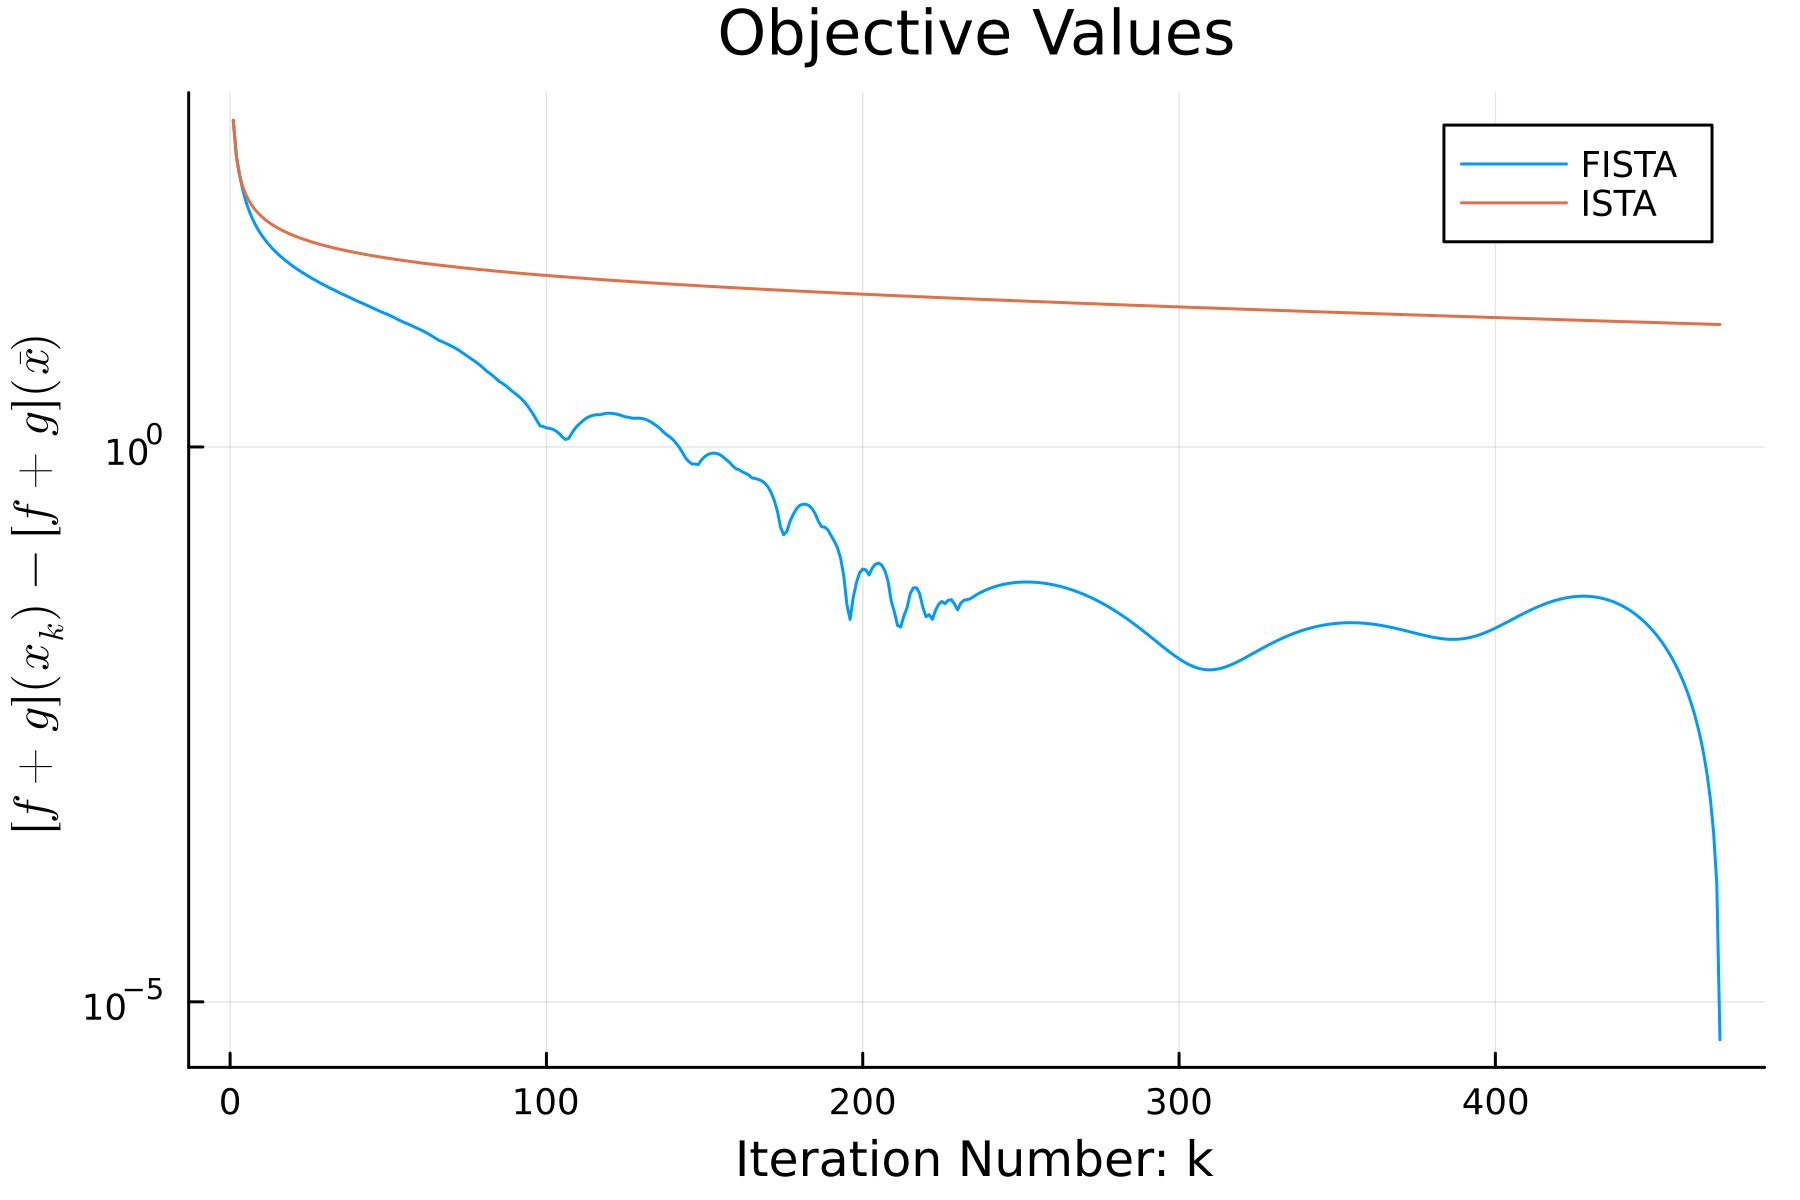
\includegraphics[width=8cm]{simple_lass_obj.png}
                \caption{The left is the objective value of the function during all iterations.}
            \end{figure}
        \end{frame}
        \begin{frame}{Results}
            The plot of $\Vert y^{(k)} - x^{(k + 1)}\Vert_\infty$:
            \begin{figure}[h]
                \centering
                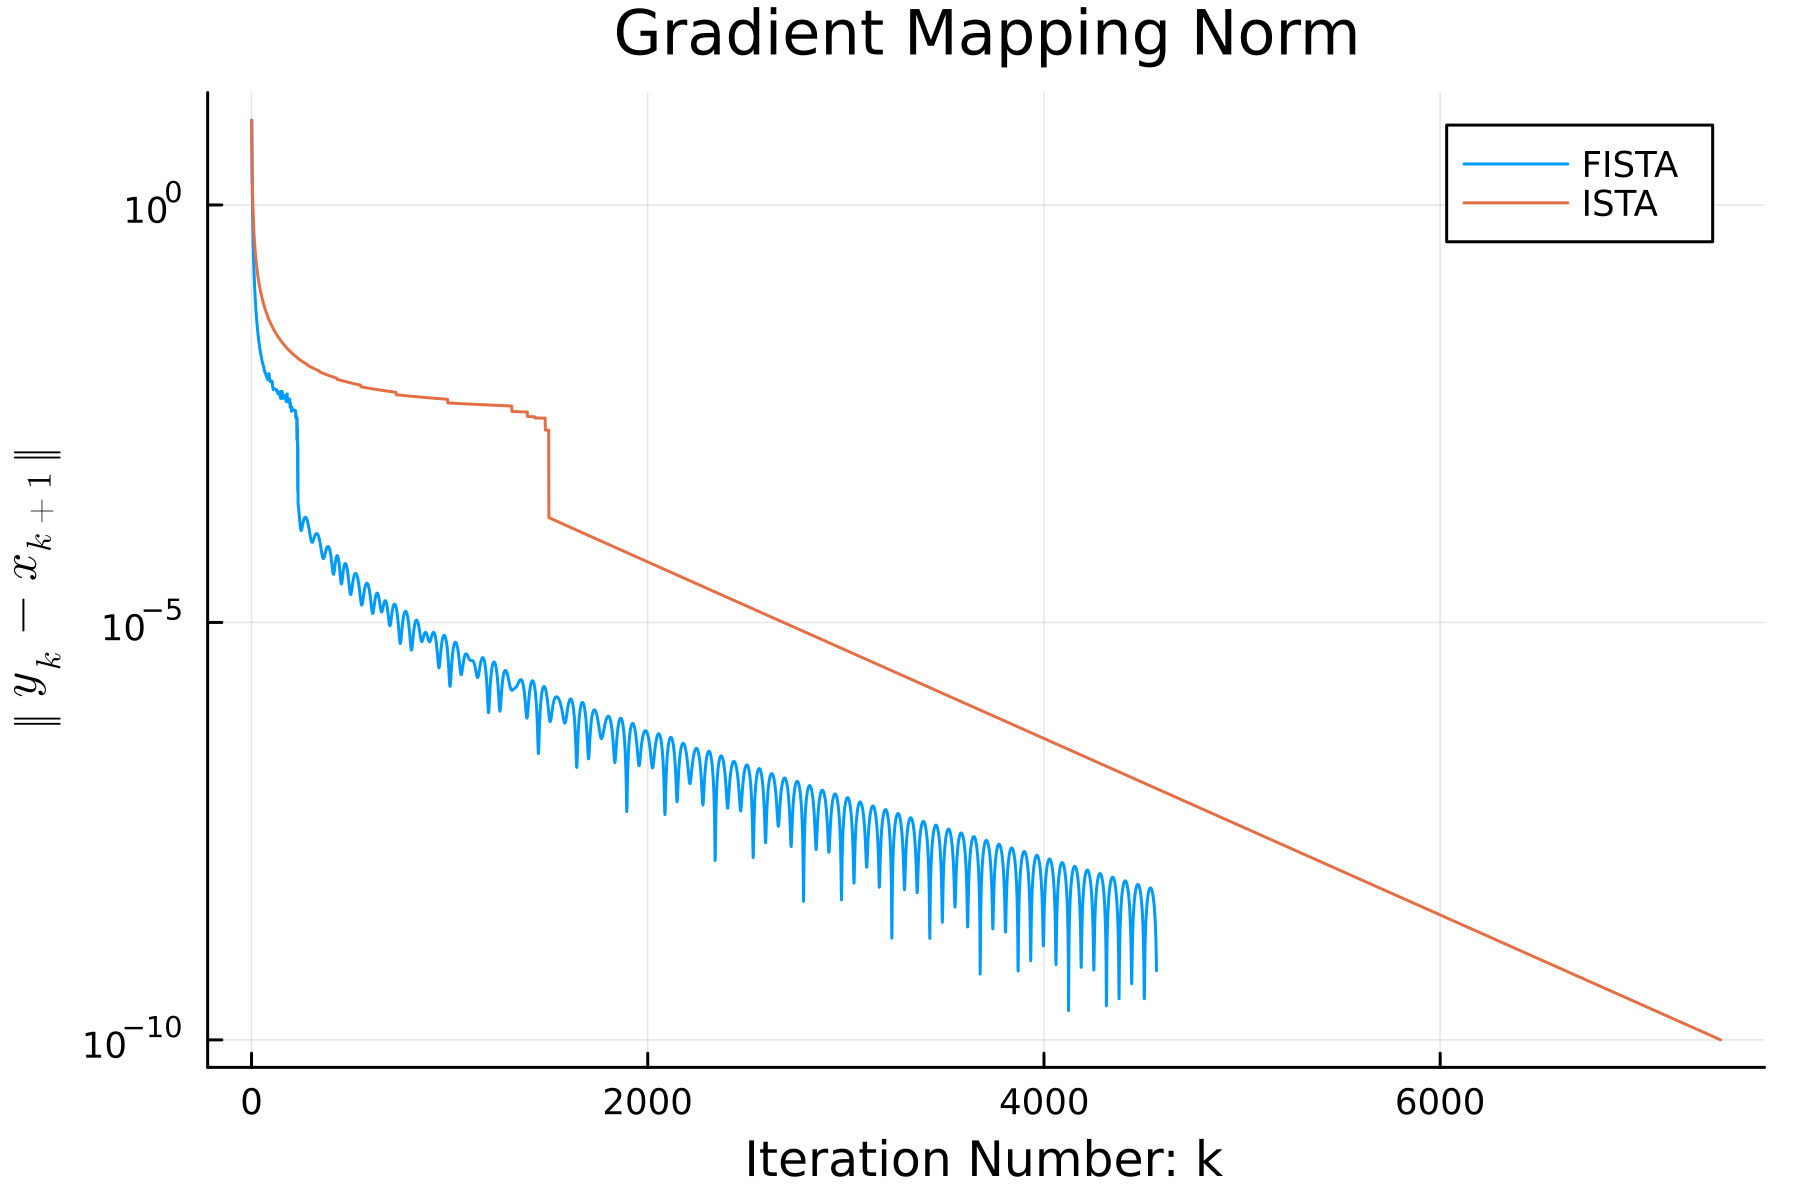
\includegraphics[width=8cm]{simple_lass_pgrad.png}
            \end{figure}
        \end{frame}
    \subsection{Image Deconvolution with Noise}
        \begin{frame}{Experiment Setup}
            Given an image that is convoluted by a Guassian kernel with some guassian noise, we want to recover the image, given the parameters for convolutions. 
            \begin{itemize}
                \item [1.] Guassian blur with a discrete 15 by 15 kernel is a linear transform represented by a sparse matrix $A$ in the computer. 
                \item [2.] When an image is 500 by 500 with three color channels, $A$ is $750000 \times 750000$. 
                \item [3.] Let the noise be on all normalized colors values with $N(0, 10^{-2})$
                \item [4.] We let $\lambda = \alpha\times (3\times500^2)^{-1}$. 
                \item [5.] Implemented in Julia, the code is too long to be shown here. 
            \end{itemize}        
        \end{frame}
        \begin{frame}{The Blurred Image}
            We consider blurring the image of a pink unicorn that I own. 
            \begin{figure}[H]
                \centering
                
\includegraphics[width=5cm]{blurred_img.jpg}
                \caption{The image is blurred by the Gaussian Blurred matrix $A$ with a tiny amount of noise on the level of $2\times 10^{-2}$ that is barely observable. Zoom in to observe the tiny amount of Gaussian noise on top of the blur.}
                \label{fig:blurred_alto}
            \end{figure}
        \end{frame}
        \begin{frame}{Results}
            \begin{figure}[H]
                \centering
                \begin{subfigure}{3.5cm}
                    
\includegraphics[width=3cm]{inverse_linear_experiment1-soln_img.jpg}
                    \caption{} \label{fig:1a}
                \end{subfigure}     %
                % \hspace*{\fill}     % maximize separation between the subfigures
                \begin{subfigure}{3.5cm}
                    
\includegraphics[width=3cm]{inverse_linear_experiment2-soln_img.jpg}
                    \caption{} \label{fig:1b}
                \end{subfigure}     %
                % \hspace*{\fill}     % maximize separation between the subfigures
                \begin{subfigure}{3.5cm}
                    
\includegraphics[width=3cm]{inverse_linear_experiment3-soln_img.jpg}
                    \caption{} \label{fig:1c}
                \end{subfigure}
                \caption{(a) $\alpha = 0$, without any one norm penalty, is not robust to the additional noise. (b) $\alpha = 0.01$, there is a tiny amount of $\lambda$. (c) $\alpha = 0.1$, it is more penalty compared to (a).}
                \label{fig:alto_deblurred}
            \end{figure}
        \end{frame}

    


\section{References}
    \begin{frame}{References}
        \bibliography{refs.bib}
    \end{frame}
\end{document}